% $Header: /cvsroot/latex-beamer/latex-beamer/solutions/conference-talks/conference-ornate-20min.en.tex,v 1.6 2004/10/07 20:53:08 tantau Exp $

\documentclass{beamer}
%\documentclass[handout]{beamer}
%\usepackage{pgfpages}
%\pgfpagesuselayout{2 on 1}[a4paper,border shrink=5mm]

% This file is a solution template for:

% - Talk at a conference/colloquium.
% - Talk length is about 20min.
% - Style is ornate.



% Copyright 2004 by Till Tantau <tantau@users.sourceforge.net>.
%
% In principle, this file can be redistributed and/or modified under
% the terms of the GNU Public License, version 2.
%
% However, this file is supposed to be a template to be modified
% for your own needs. For this reason, if you use this file as a
% template and not specifically distribute it as part of a another
% package/program, I grant the extra permission to freely copy and
% modify this file as you see fit and even to delete this copyright
% notice.


\mode<presentation>
{
%  \usetheme{Warsaw}
%  \usetheme{Boadilla}
%  \usetheme{Goettingen}
%  \usetheme{Hannover}
%  \usetheme{Madrid}
%  \usetheme{Marburg}
%  \usetheme{Montpellier}
%  \usetheme{Pittsburgh}
  \usetheme{Hawke}
  % or ...

  \setbeamercovered{transparent}
  % or whatever (possibly just delete it)
}


\usepackage[english]{babel}
% or whatever

\usepackage[latin1]{inputenc}
% or whatever

\usepackage{times}
\usepackage[T1]{fontenc}
% Or whatever. Note that the encoding and the font should match. If T1
% does not look nice, try deleting the line with the fontenc.

\usepackage{multimedia}


%%%%%%
% My Commands
%%%%%%

\newcommand{\ml}{{\sc matlab}}
\newcommand{\bb}{{\boldsymbol{b}}}
\newcommand{\bx}{{\boldsymbol{x}}}
\newcommand{\by}{{\boldsymbol{y}}}
\newcommand{\bfm}[1]{{\boldsymbol{#1}}}

%%%%

\title[Lecture 12] % (optional, use only with long paper titles)
{Lecture 12 - Quadrature}

% \subtitle
% {Include Only If Paper Has a Subtitle}

\author[I. Hawke] % (optional, use only with lots of authors)
{I.~Hawke}
% - Give the names in the same order as the appear in the paper.
% - Use the \inst{?} command only if the authors have different
%   affiliation.

\institute[University of Southampton] % (optional, but mostly needed)
{
%  \inst{1}%
  School of Mathematics, \\
  University of Southampton, UK
}
% - Use the \inst command only if there are several affiliations.
% - Keep it simple, no one is interested in your street address.

\date[Semester 1] % (optional, should be abbreviation of conference name)
{MATH3018/6141, Semester 1}
% - Either use conference name or its abbreviation.
% - Not really informative to the audience, more for people (including
%   yourself) who are reading the slides online

\subject{Numerical methods}
% This is only inserted into the PDF information catalog. Can be left
% out.



% If you have a file called "university-logo-filename.xxx", where xxx
% is a graphic format that can be processed by latex or pdflatex,
% resp., then you can add a logo as follows:

\pgfdeclareimage[height=0.5cm]{university-logo}{mathematics_7469}
\logo{\pgfuseimage{university-logo}}



% Delete this, if you do not want the table of contents to pop up at
% the beginning of each subsection:
%  \AtBeginSubsection[]
%  {
%    \begin{frame}<beamer>
%      \frametitle{Outline}
%      \tableofcontents[currentsection,currentsubsection]
%    \end{frame}
%  }
\AtBeginSection[]
{
  \begin{frame}<beamer>
    \frametitle{Outline}
    \tableofcontents[currentsection]
  \end{frame}
}


% If you wish to uncover everything in a step-wise fashion, uncomment
% the following command:

%\beamerdefaultoverlayspecification{<+->}


\begin{document}

\begin{frame}
  \titlepage
\end{frame}

\section{Quadrature}

\subsection{Quadrature}

\begin{frame}
  \frametitle{Numerical Quadrature}

  The aim of numerical quadrature is to compute
  \begin{equation*}
    \int_a^b f(x) \, \text{d}x
  \end{equation*}
  where $f$ is a real function of a single variable $x$. \pause

  \vspace{1ex}

  More complex integrals are best evaluated by analytical reduction to
  a (set of) integral(s) in the form above. \pause

  \vspace{1ex}

  Here we will always assume that $f(x)$ is finite within $[a, b]$,
  and frequently we will implicitly assume that it is differentiable.

\end{frame}

\begin{frame}
  \frametitle{The simplest quadrature}

  \begin{columns}
    \begin{column}{0.5\textwidth}
      Standard situation: the value of the function is known (or can
      be evaluated) at a set of points or \emph{nodes}. \pause

      \vspace{1ex}

      The simplest evaluation of the quadrature uses the Riemann
      integral: a rectangular area is computed for each node, and the
      total integral is the sum of these areas.
    \end{column}
    \begin{column}{0.5\textwidth}
      \begin{overlayarea}{\textwidth}{0.5\textheight}
        \only<1|handout:1>
        {
          \begin{center}
            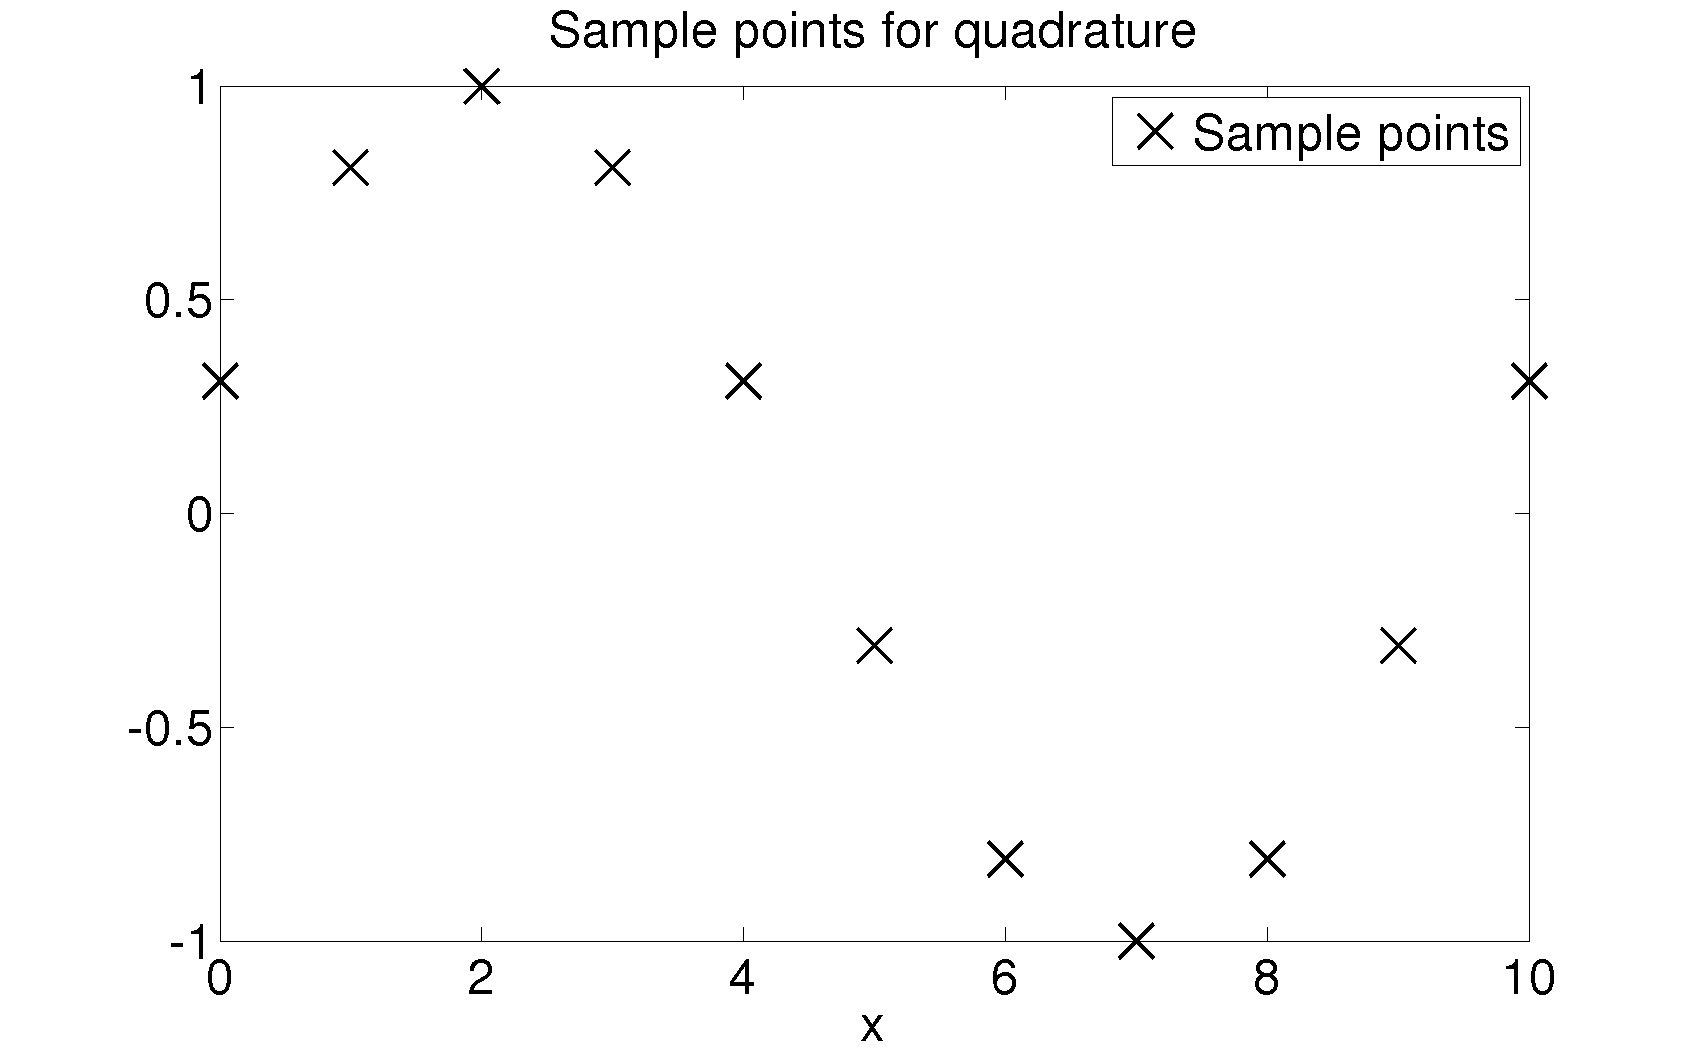
\includegraphics[width=\textwidth]{figures/QuadAliasing1}
          \end{center}
        }
        \only<2|handout:2>
        {
          \begin{center}
            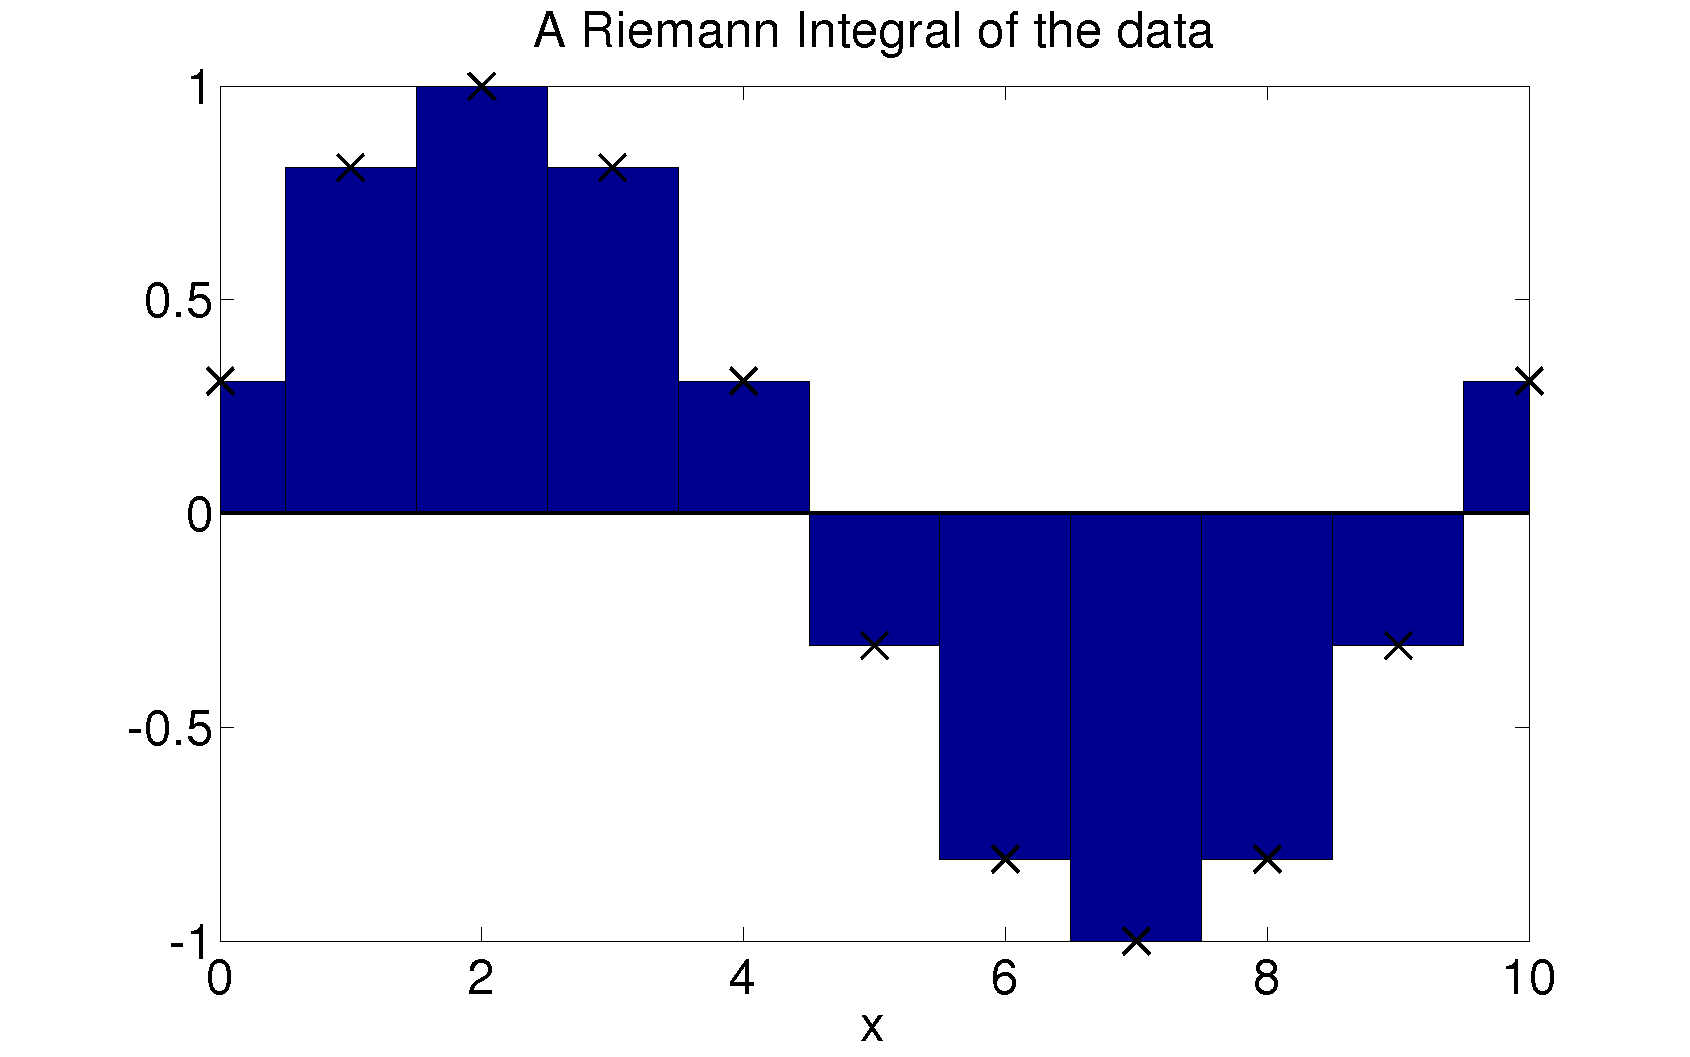
\includegraphics[width=\textwidth]{figures/QuadRiemann1}
          \end{center}
        }
      \end{overlayarea}
    \end{column}
  \end{columns}

\end{frame}


\subsection{Function representation}

\begin{frame}
  \frametitle{Function representation}

  The simple rule from the Riemann integral is not very accurate. Most
  improvements change how the function is represented using a finite
  amount of information. \pause

  \vspace{1ex}

  \begin{columns}
    \begin{column}{0.5\textwidth}
      \begin{overlayarea}{\textwidth}{0.6\textheight}
        \only<2-5|handout:1-4>
        {
          Simplest assumption: know the \emph{values} $f(x_j)$ at
          nodes $x_j$. This does not give us complete information
          about the function.

          \vspace{1ex}
        }
        \only<3|handout:2>
        {

          We need information about how the function behaves away from
          the nodes. We \emph{assume} the function behaves in a
          suitably simple way, so that the resulting
          \emph{interpolating function} is easy to use.
        }
        \only<4|handout:3>
        {

          If the interpolating function is integrable then we are
          done; compute the integrals between each node and sum.
        }
        \only<5|handout:4>
        {

          The choice of interpolating function is definitely not
          unique. With quadrature this is not so much of an issue.
        }
        \only<6-7|handout:5>
        {
          A different assumption is that we can compute the function
          at any point in the interval, but that we wish to do this as
          little as possible.

        }
        \only<7|handout:5>
        {
          \vspace{1ex}
          We then pick the nodes and the interpolating function to
          get the highest degree of accuracy possible. If the nodes
          are chosen based on the values of the function $f$ itself
          then this is an \emph{adaptive} algorithm.
        }
        \only<8|handout:6>
        {
          Another possibility is that we might know (or compute) the
          coefficients of the function with respect to some basis,
          such as the Fourier coefficients
          \begin{equation*}
            f(x) \simeq \sum_{n=1}^N a_n \sin \left(\frac{2 \pi n}{L}
              x\right).
          \end{equation*}
        }
        \only<9|handout:7>
        {
          \begin{equation*}
            f(x) \simeq \sum_{n=1}^N a_n \sin \left(\frac{2 \pi n}{L}
              x\right).
          \end{equation*}

          Use linearity to compute the integral of each
          basis function, and compute the total integral using the
          appropriate weighted sum.
        }
      \end{overlayarea}
    \end{column}
    \begin{column}{0.5\textwidth}
      \begin{overlayarea}{\textwidth}{0.6\textheight}
        \only<2|handout:1>
        {
          \begin{center}
            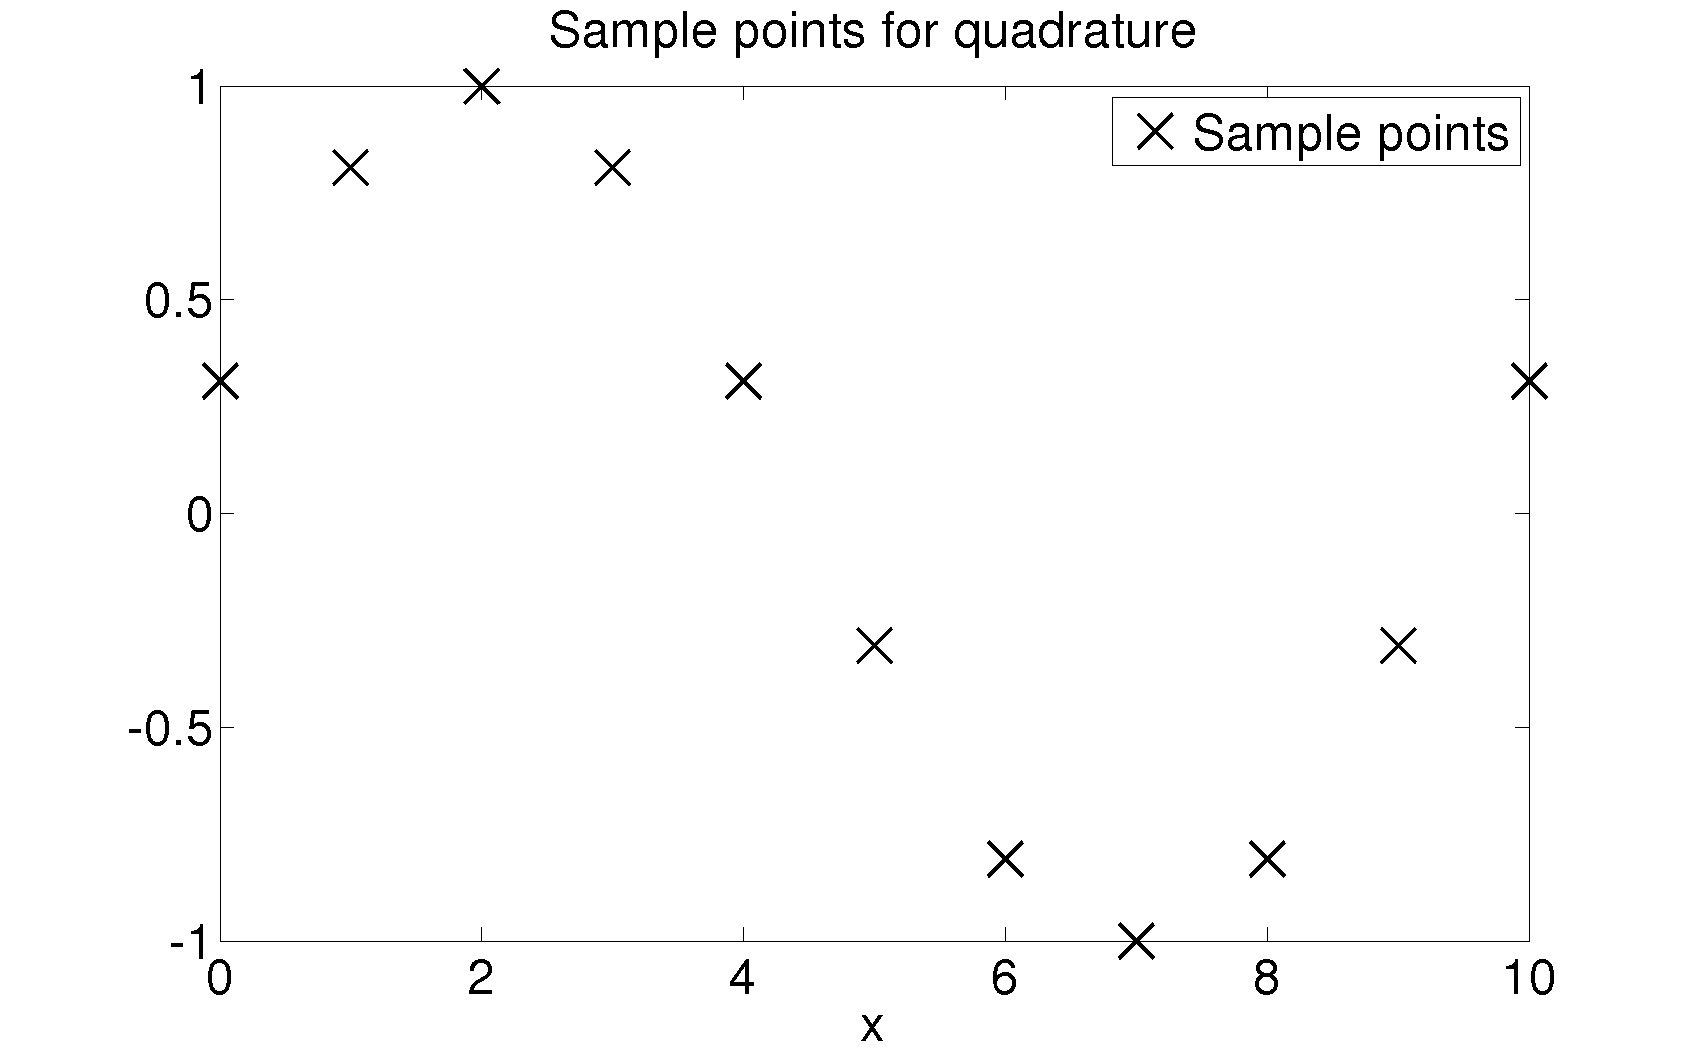
\includegraphics[width=\textwidth]{figures/QuadAliasing1}
          \end{center}
        }
        \only<3|handout:2>
        {
          \begin{center}
            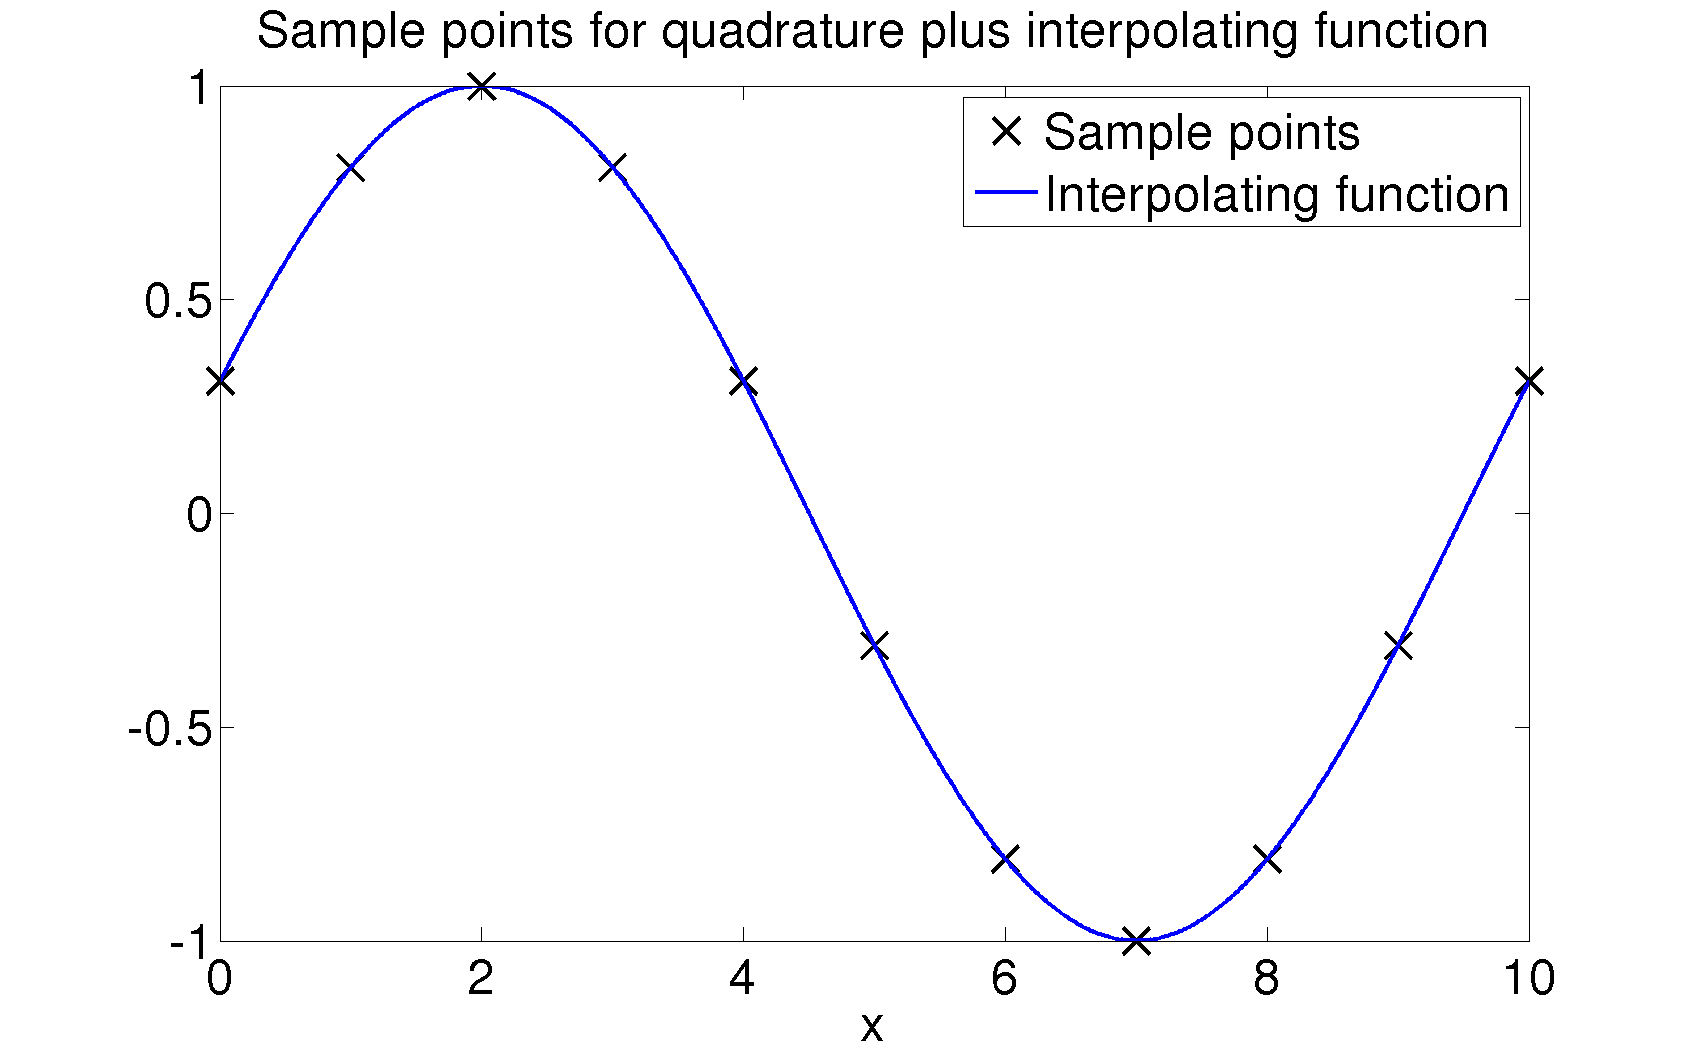
\includegraphics[width=\textwidth]{figures/QuadAliasing2}
          \end{center}
        }
        \only<4|handout:3>
        {
          \begin{center}
            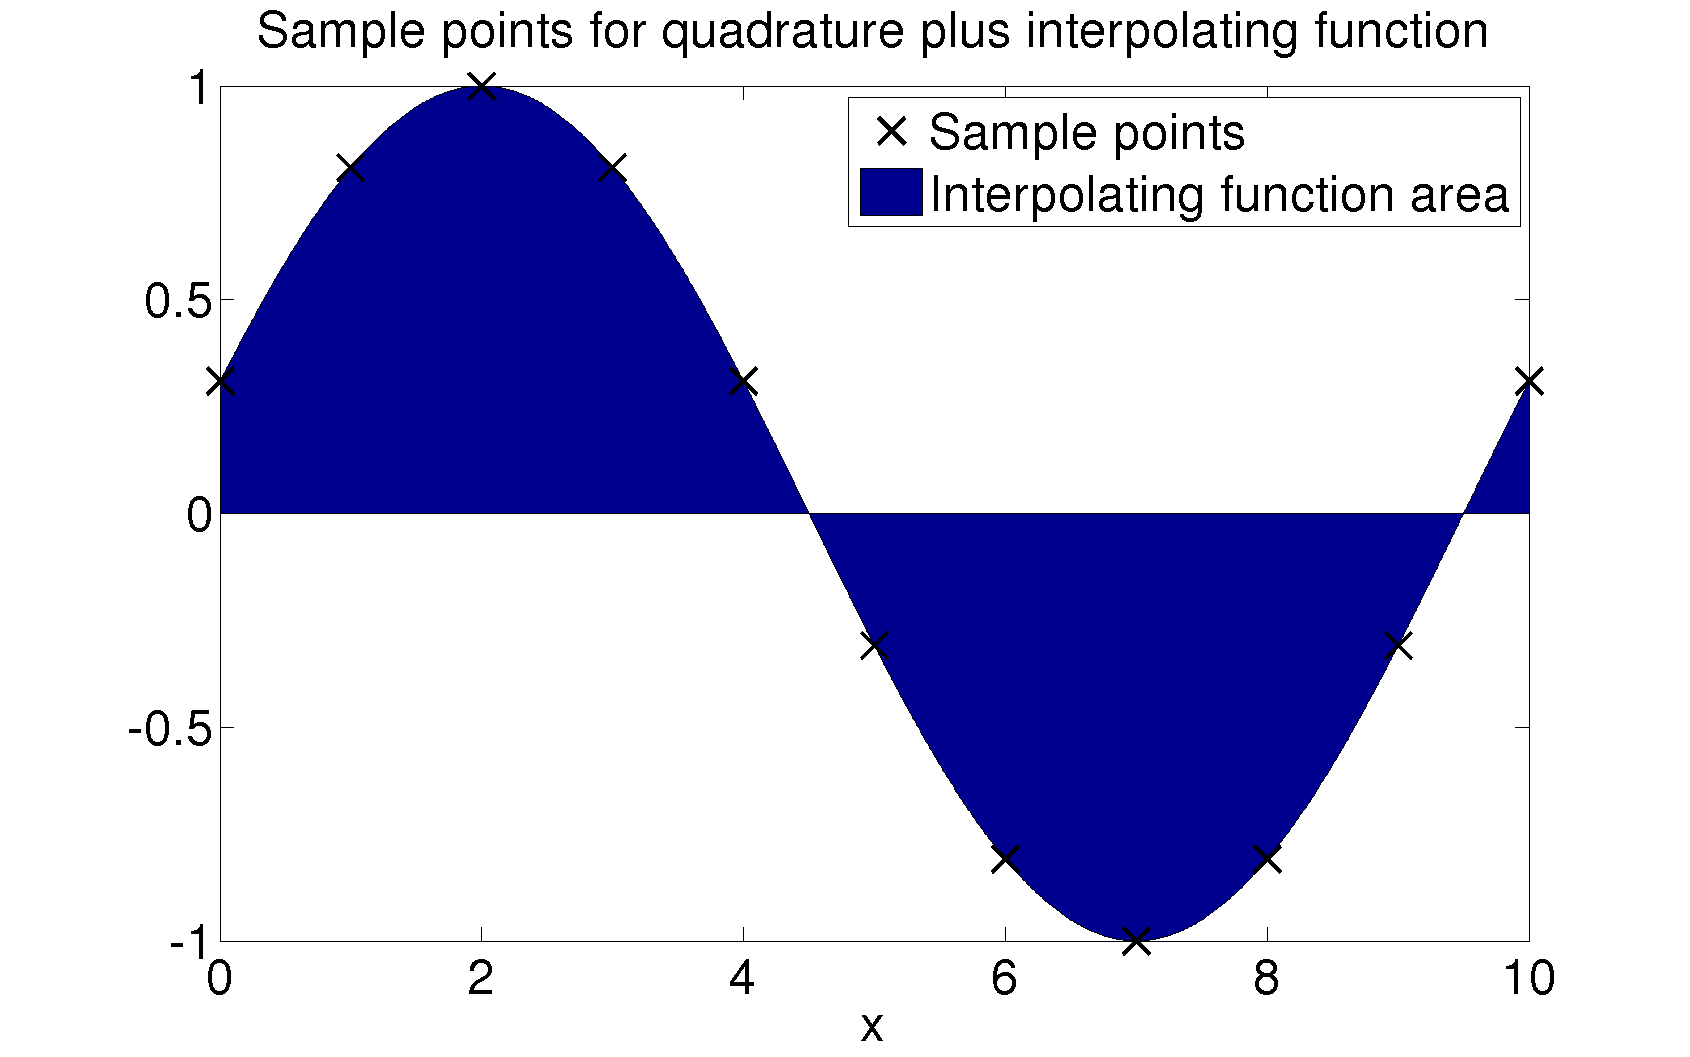
\includegraphics[width=\textwidth]{figures/QuadAliasing3}
          \end{center}
        }
        \only<5|handout:4>
        {
          \begin{center}
            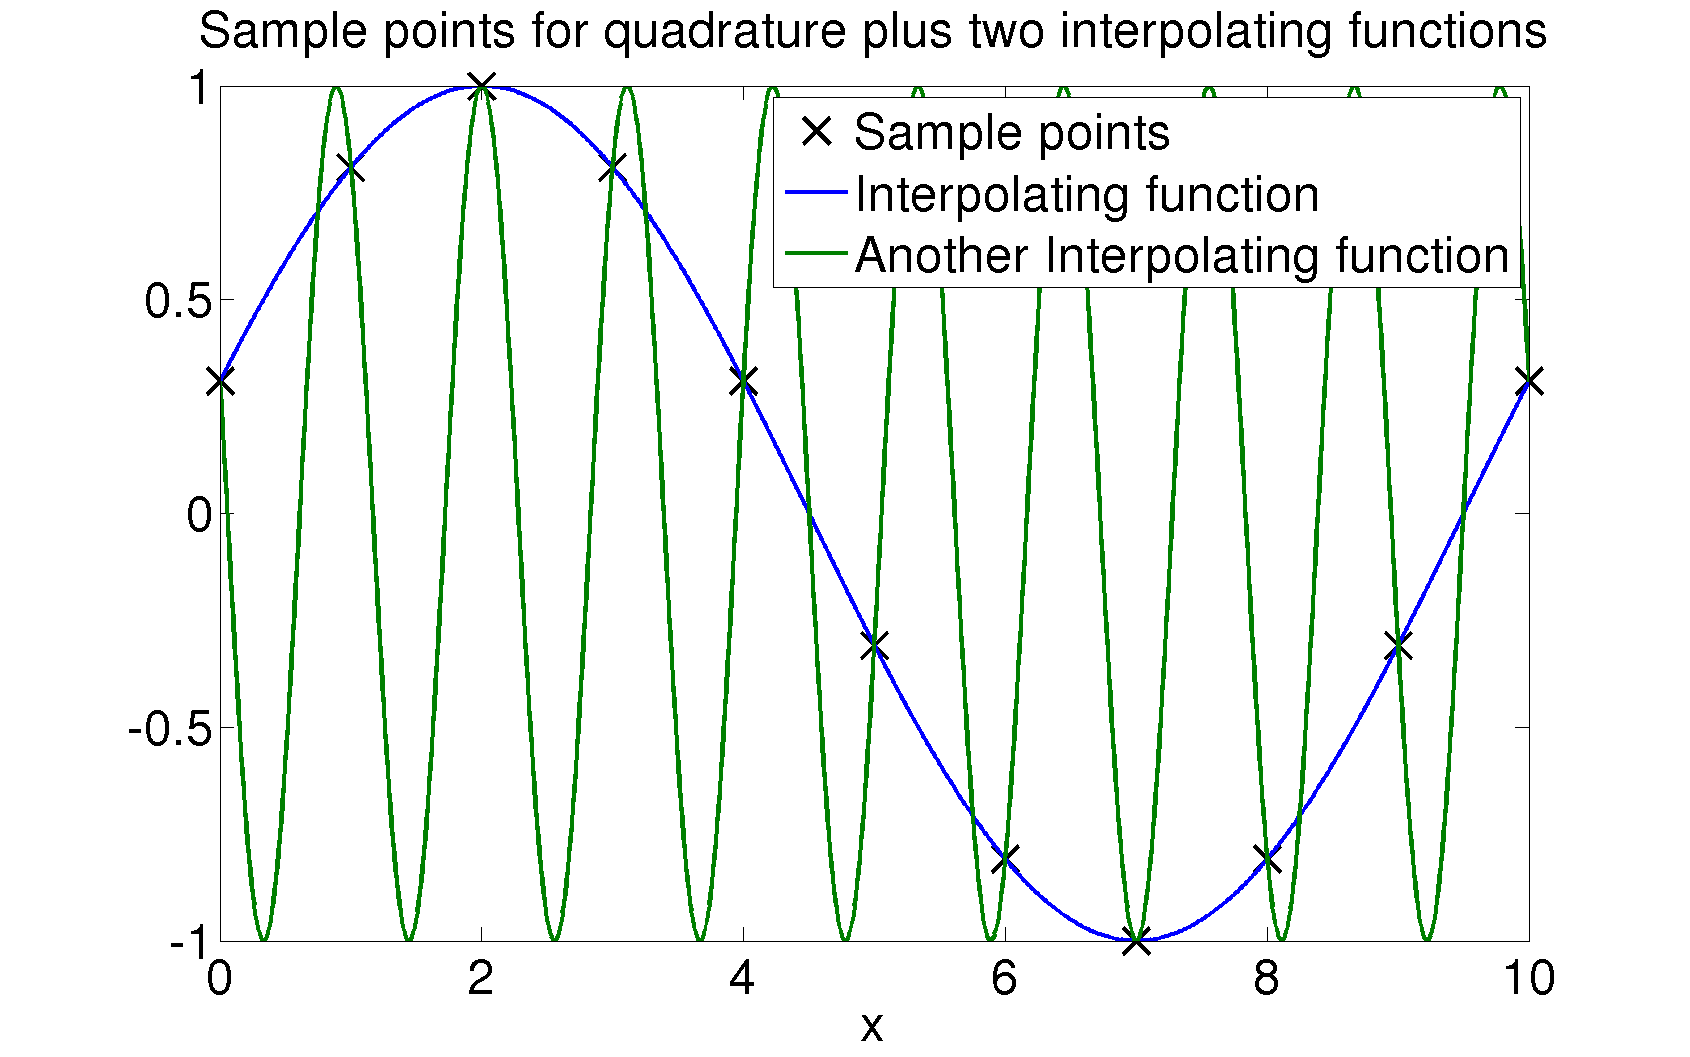
\includegraphics[width=\textwidth]{figures/QuadAliasing4}
          \end{center}
        }
        \only<6|handout:0>
        {
          \begin{center}
            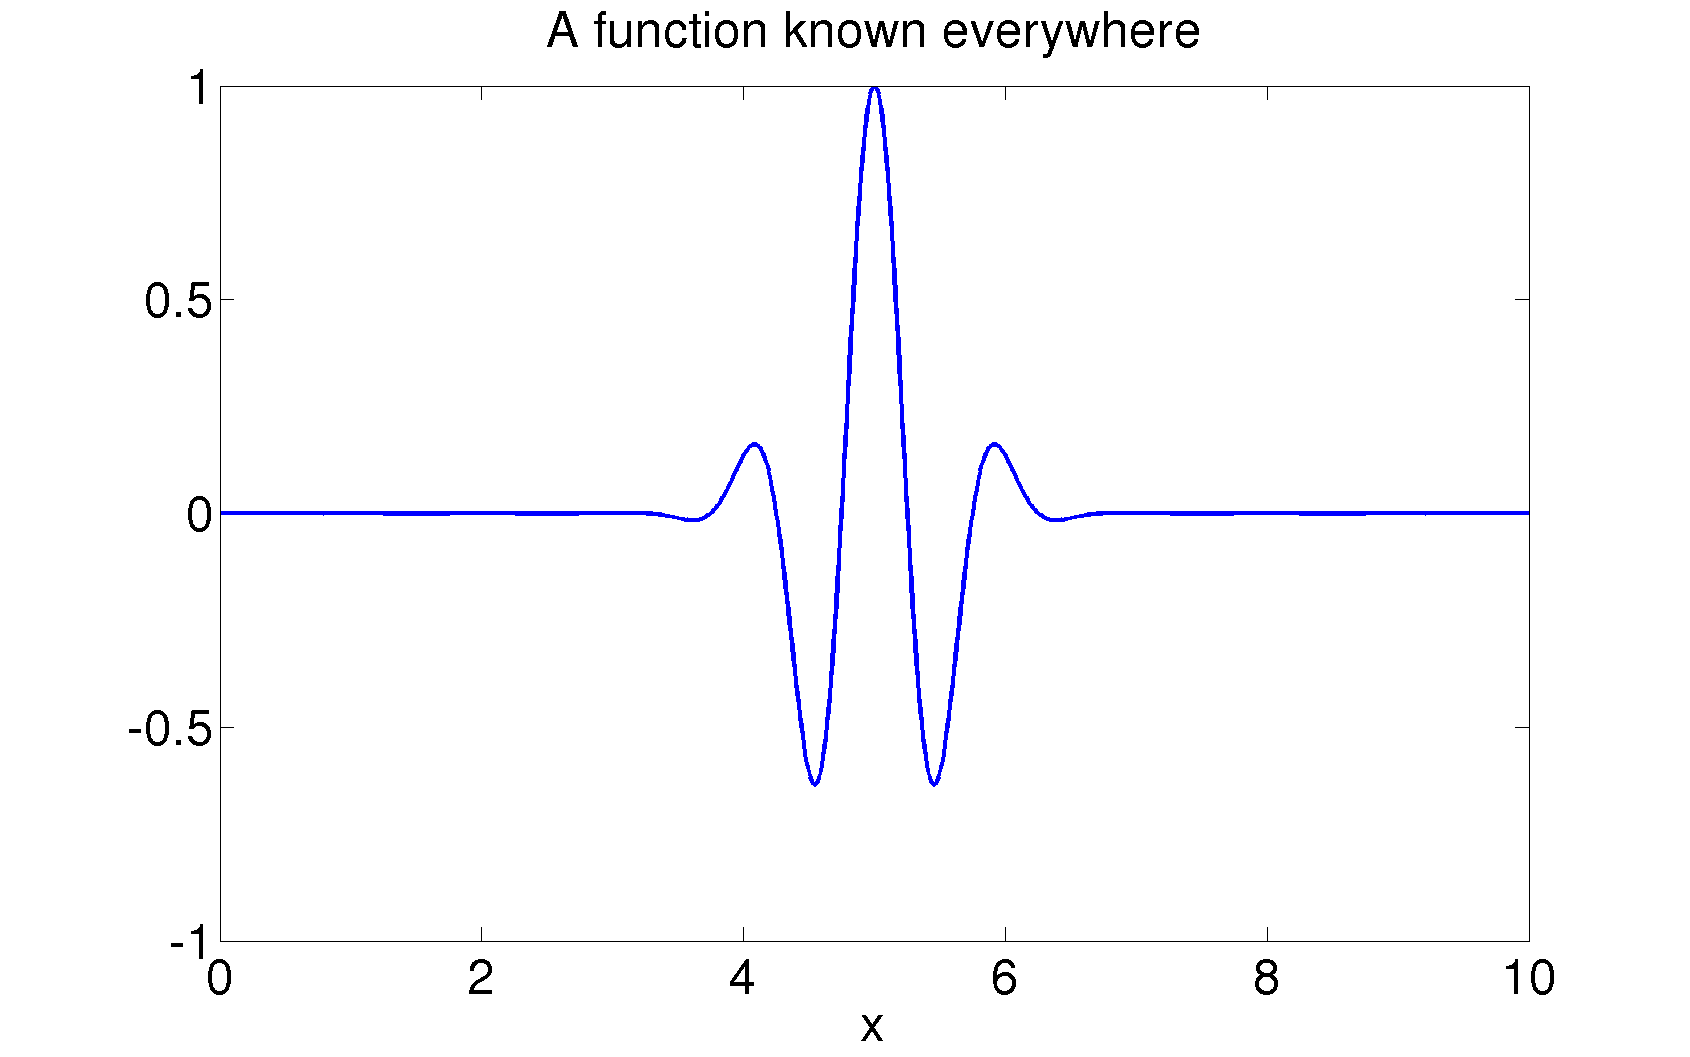
\includegraphics[width=\textwidth]{figures/QuadAdaptive1}
          \end{center}
        }
        \only<7|handout:5>
        {
          \begin{center}
            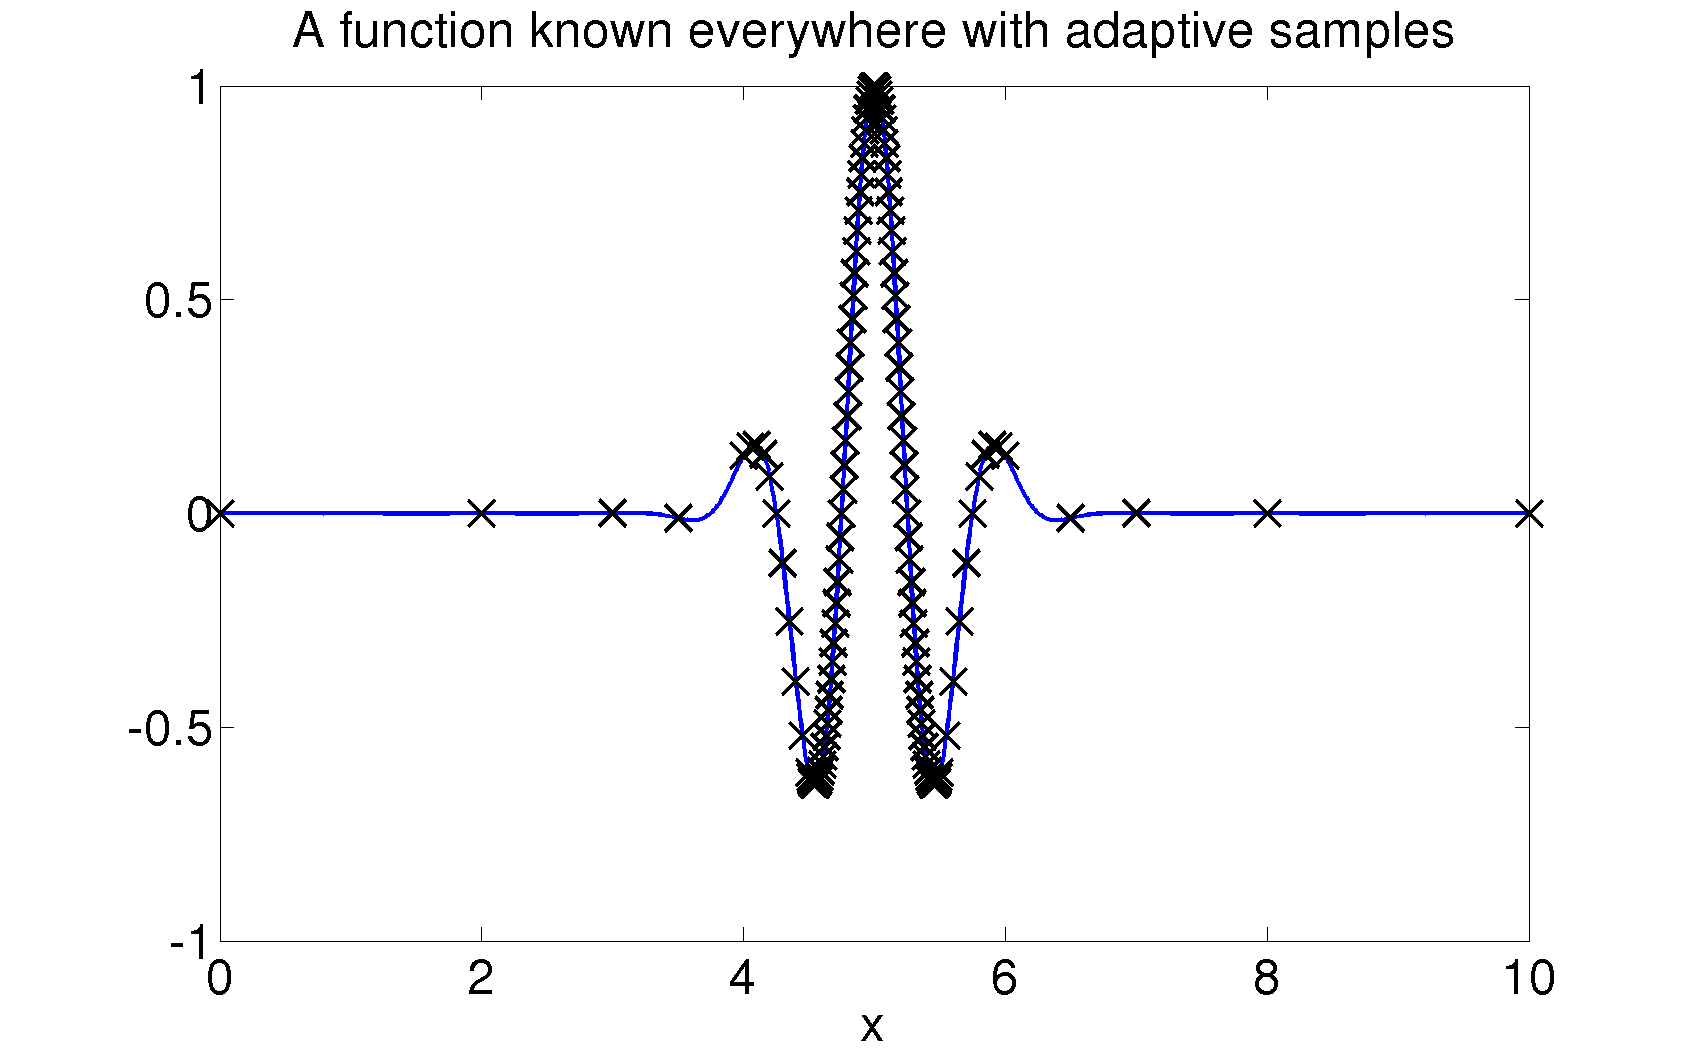
\includegraphics[width=\textwidth]{figures/QuadAdaptive2}
          \end{center}
        }
        \only<8-9|handout:6-7>
        {
          \begin{center}
            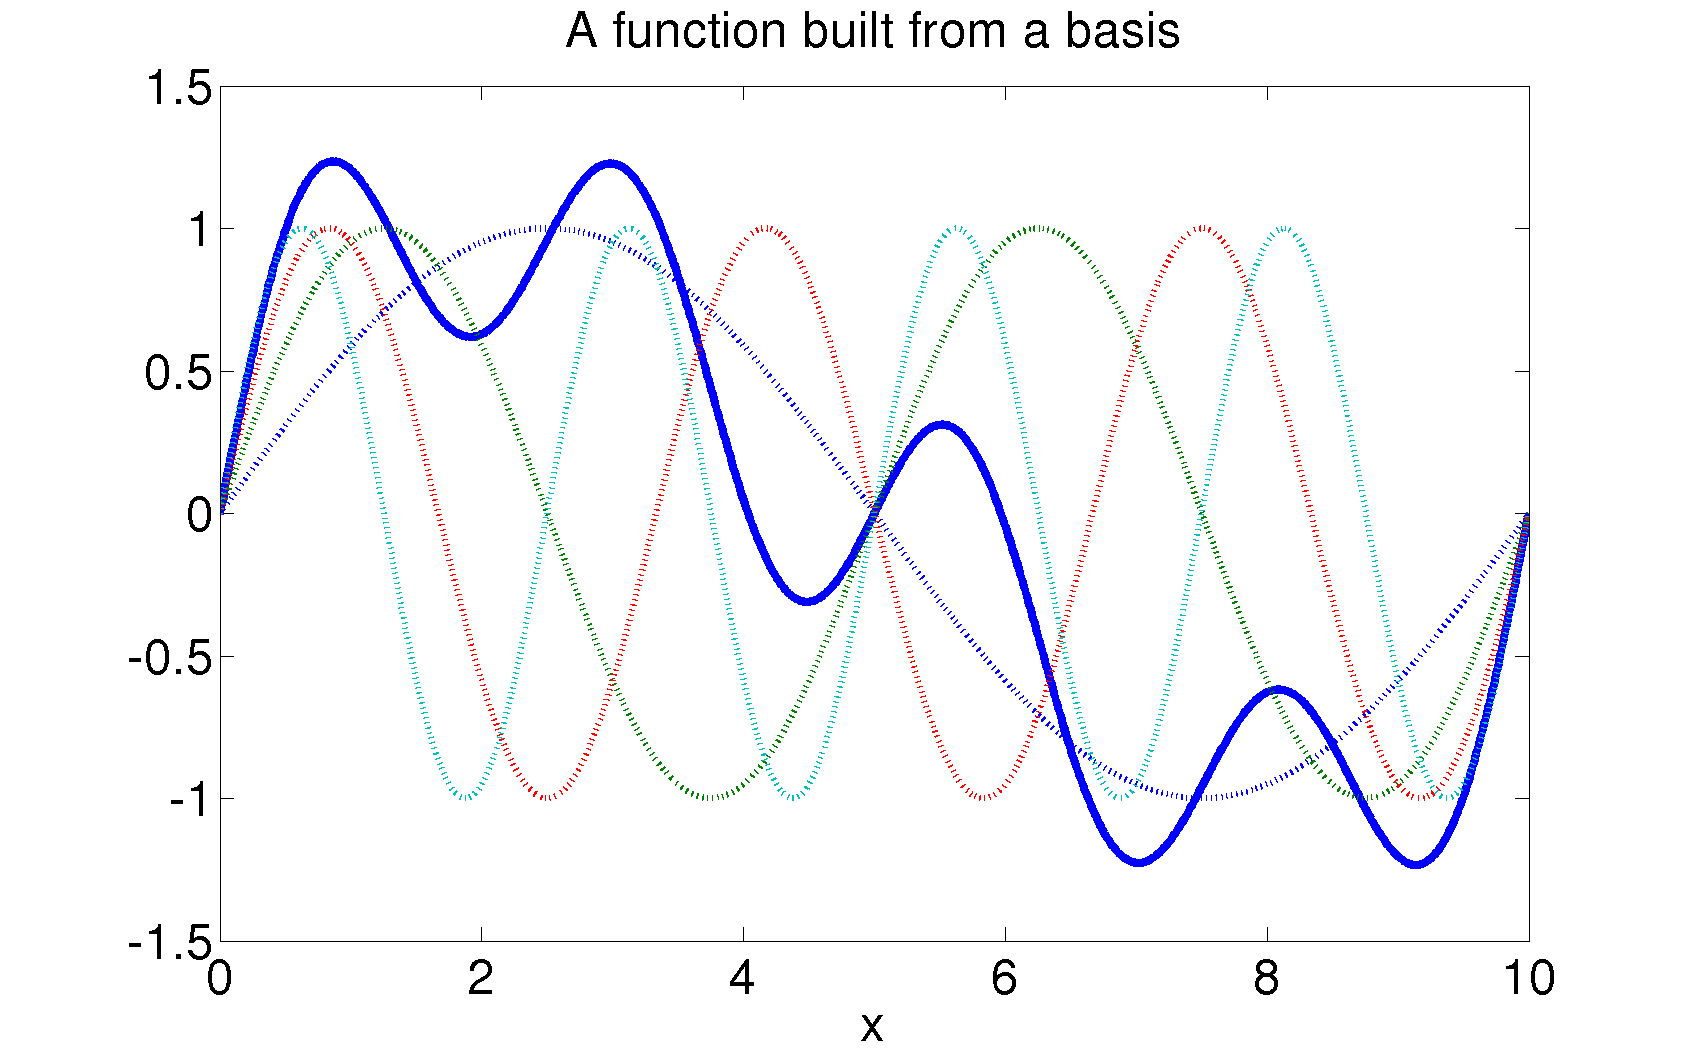
\includegraphics[width=\textwidth]{figures/QuadBasis1}
          \end{center}
        }
      \end{overlayarea}
    \end{column}
  \end{columns}

\end{frame}


\subsection{Polynomial interpolation}

\begin{frame}
  \frametitle{Polynomial interpolation}

  The general class of methods that have the name of
  \emph{Newton-Cotes} formulae are simple and robust. They make the
  following assumptions:
  \begin{itemize}
  \item The function $f(x)$ is known (or can be evaluated) at a finite
    set of nodes $\{x_j\}$, with $j = 0, \dots, N$, in the interval
    $[a, b]$. \pause
  \item An interpolating function $g(x)$ is found that passes through
    these points, i.e.\
    \begin{equation*}
      g(x_j) = f(x_j) \left( = f_j \right), \quad j = 0, \dots, N.
    \end{equation*} \pause
  \item The interpolating function is a polynomial or piecewise
    polynomial. \pause
  \item The integral is computed from the exact integral of $g(x)$
    over the interval.
  \end{itemize} \pause

  Different methods based on the order of the polynomials used and
  restrictions on the nodes.

\end{frame}


\subsection{Trapezoidal rule}


\begin{frame}
  \frametitle{Trapezoidal rule}

  The trapezoidal rule uses an interpolating polynomial $g(x)$ of
  order 1: a straight line.
  \begin{columns}
    \begin{column}{0.5\textwidth}
      \begin{overlayarea}{\textwidth}{0.7\textheight}
        \only<2-3|handout:1>
        {
          \vspace{1ex}
          Hence
          \begin{equation*}
            \int_a^b f(x) \, \text{d}x = \tfrac{1}{2} (b - a) \left[ f(b) +
              f(a) \right].
          \end{equation*}
        }
        \only<3|handout:1>
        {

          Very inaccurate unless the interval is small or $f(x)$ is
          very boring.
        }
        \only<4-5|handout:2>
        {
          \vspace{1ex}
          Instead use the \emph{composite} trapezoidal rule. Divide
          interval into $N$ equal subintervals length
          \begin{equation*}
            h = (b - a) / N,
          \end{equation*}
          and apply trapezoidal rule to each.
        }
        \only<5|handout:2>
        {
          Resulting interpolation polynomial $g$ is
          \emph{piecewise} linear. Area in each subinterval is
          \begin{equation*}
            A_j = \tfrac{1}{2} (x_j - x_{j-1}) \left[ f(x_j) + f(x_{j-1})
            \right].
          \end{equation*}
        }
      \end{overlayarea}
    \end{column}
    \begin{column}{0.5\textwidth}
      \begin{overlayarea}{\textwidth}{0.7\textheight}
        \only<2-3|handout:1>
        {
          \begin{center}
            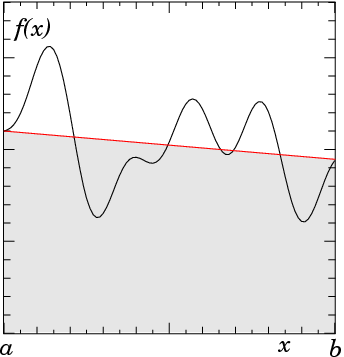
\includegraphics[width=\textwidth]{figures/trapez1}
          \end{center}
        }
        \only<4-5|handout:2>
        {
          \begin{center}
            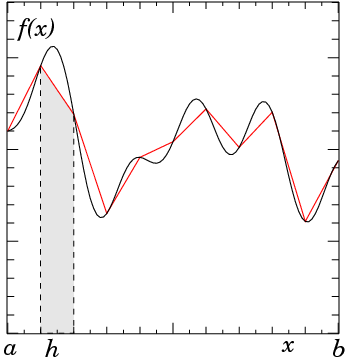
\includegraphics[width=\textwidth]{figures/trapez2}
          \end{center}
        }
      \end{overlayarea}
    \end{column}
  \end{columns}
\end{frame}

 \begin{frame}
   \frametitle{Composite Trapezoidal Rule}


   \begin{columns}
      \begin{column}{0.5\textwidth}
        \begin{overlayarea}{\textwidth}{0.7\textheight}
          \only<1->
          {
            From each subinterval the area is
            \begin{equation*}
              A_j = \tfrac{1}{2} (x_j - x_{j-1}) \left[ f(x_j) + f(x_{j-1})
              \right]
            \end{equation*}
            and we obtain the full answer by summing each segment to get
            \begin{equation*}
              \int_a^b f(x)\, \text{d}x = \tfrac{h}{2} \sum_{j=1}^N
              \left[ f_j + f_{j-1} \right]
            \end{equation*}
          }
          \only<2>
          {

            This is often written as
            \begin{align*}
              \int_a^b f(x)\, \text{d}x& = \tfrac{h}{2} \left(f_0 +
                f_N\right) \\&+ h \left(f_1 + \dots f_{N-1} \right).
            \end{align*}
          }
        \end{overlayarea}
      \end{column}
     \begin{column}{0.5\textwidth}
       \begin{center}
         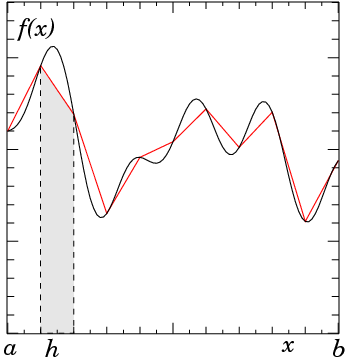
\includegraphics[width=\textwidth]{figures/trapez2}
       \end{center}
     \end{column}
   \end{columns}

 \end{frame}


 \subsection{Error analysis}


 \begin{frame}
   \frametitle{Errors: 1}

   To compute the error from a composite quadrature rule we bound the
   error in any subinterval. This will depend on the width of the
   interval, $h$. \pause

   \vspace{1ex}

   We firstly write the trapezoidal rule on one interval as
   \begin{equation*}
     A_j = \tfrac{h}{2} \left(f_j + f_{j+1}\right).
   \end{equation*} \pause
   If we Taylor expand $f_{j+1}$ about $f_j$ we have
   \begin{equation*}
     A_j = h f_j + \tfrac{h^2}{2} f'_j + \tfrac{h^3}{4} f^{(2)}_j + \dots
   \end{equation*}
 \end{frame}

 \begin{frame}
   \frametitle{Errors: 2}

   To find the error, we need the exact result in powers of $h$. So define
   \begin{equation*}
     F(t) = \int_{x_j}^{x_j + t} f(x) \, \text{d}x
   \end{equation*}
   so that
   \begin{equation*}
     F(h) = \int_{x_j}^{x_{j+1}} f(x) \, \text{d}x.
   \end{equation*}
   We note that
   \begin{equation*}
     \frac{\text{d}^n F}{\text{d}t^n} = f^{(n-1)}(x_j + t)
   \end{equation*}
   or in particular
   \begin{equation*}
     \frac{\text{d} F}{\text{d}t} = f(x_j + t).
   \end{equation*}
 \end{frame}

\begin{frame}
  \frametitle{Errors: 3}

  From this we can Taylor expand about $t=0$ to find
  \begin{equation*}
    F(h) = F(0) + h \left. \frac{\text{d}F}{\text{d}t} \right|_{t=0}
    + \dots
  \end{equation*} \pause
  From the definition of $\text{d}F / \text{d}t$ we have
  \begin{equation*}
    F(h) = h f_j + \tfrac{h^2}{2} f'_j + \tfrac{h^3}{6} f^{(2)}_j + \dots.
  \end{equation*} \pause
  Comparing with the trapezoidal rule
  \begin{equation*}
    F(h) \simeq A_j = h f_j + \tfrac{h^2}{2} f'_j + \tfrac{h^3}{4}
    f^{(2)}_j + \dots
  \end{equation*}
  the error in the subinterval is
  \begin{equation*}
    | A_j - F(h) | \leq \tfrac{h^3}{12} |f^{(2)}_j| .
  \end{equation*} \pause

  Summing over all $N$ subintervals and using $h N = (b - a)$ gives
  \begin{equation*}
    \text{Error} \leq \frac{(b - a) h^2}{12} M_2, \quad M_2 =
    \max_{x\in[a,b]} | f^{(2)}(x) |.
  \end{equation*}

\end{frame}

\subsection{Example}

\begin{frame}
  \frametitle{Example}

  We look at
  \begin{equation*}
    \int_0^{\pi / 2} \sin(x) \, \text{d}x
  \end{equation*}
  using the trapezoidal rule. The exact answer is 1.

  \begin{overlayarea}{\textwidth}{0.7\textheight}
    \only<2|handout:1>
    {
       With three points $x_j = \{0, \pi / 4, \pi / 2\}$ we have $h =
       \pi / 4$ and
       \begin{center}
         \begin{tabular}{c|c c}
           $j$ & $x_j$ & $f_j$ \\ \hline
           0 & 0 & 0 \\
           1 & $\pi / 4$ & $1 / \sqrt{2}$ \\
           2 & $\pi / 2$ & 1
         \end{tabular}
       \end{center}
       So
       \begin{align*}
         \int_0^{\pi / 2} \sin(x) \, \text{d}x & \simeq \frac{\pi / 4}{2}
         \left( 0 + 1 \right) + \pi / 4 \left( \tfrac{1}{\sqrt{2}} \right)
         \\
         & = \tfrac{\pi}{8} \left( 1 + \sqrt{2} \right) \\
         & \simeq 0.948.
       \end{align*}
    }
    \only<3|handout:2>
    {
      With four points $x_j = \{0, \pi / 6, \pi / 3, \pi / 2\}$ we have
      $h = \pi / 6$ and
      \begin{center}
        \begin{tabular}{c|c c}
          $j$ & $x_j$ & $f_j$ \\ \hline
          0 & 0 & 0 \\
          1 & $\pi / 6$ & $1 / 2$ \\
          2 & $\pi / 3$ & $\sqrt{3} / 2$ \\
          3 & $\pi / 2$ & 1
        \end{tabular}
      \end{center}
      So
      \begin{align*}
        \int_0^{\pi / 2} \sin(x) \, \text{d}x & \simeq \frac{\pi / 6}{2}
        \left( 0 + 1 \right) + \pi / 6 \left( \tfrac{1}{2} +
          \tfrac{\sqrt{3}}{2} \right)
        \\
        & = \tfrac{\pi}{12} \left( 2 + \sqrt{3} \right) \simeq 0.977.
      \end{align*}
    }
  \end{overlayarea}

\end{frame}

\begin{frame}
  \frametitle{Example Convergence}

  \begin{center}
    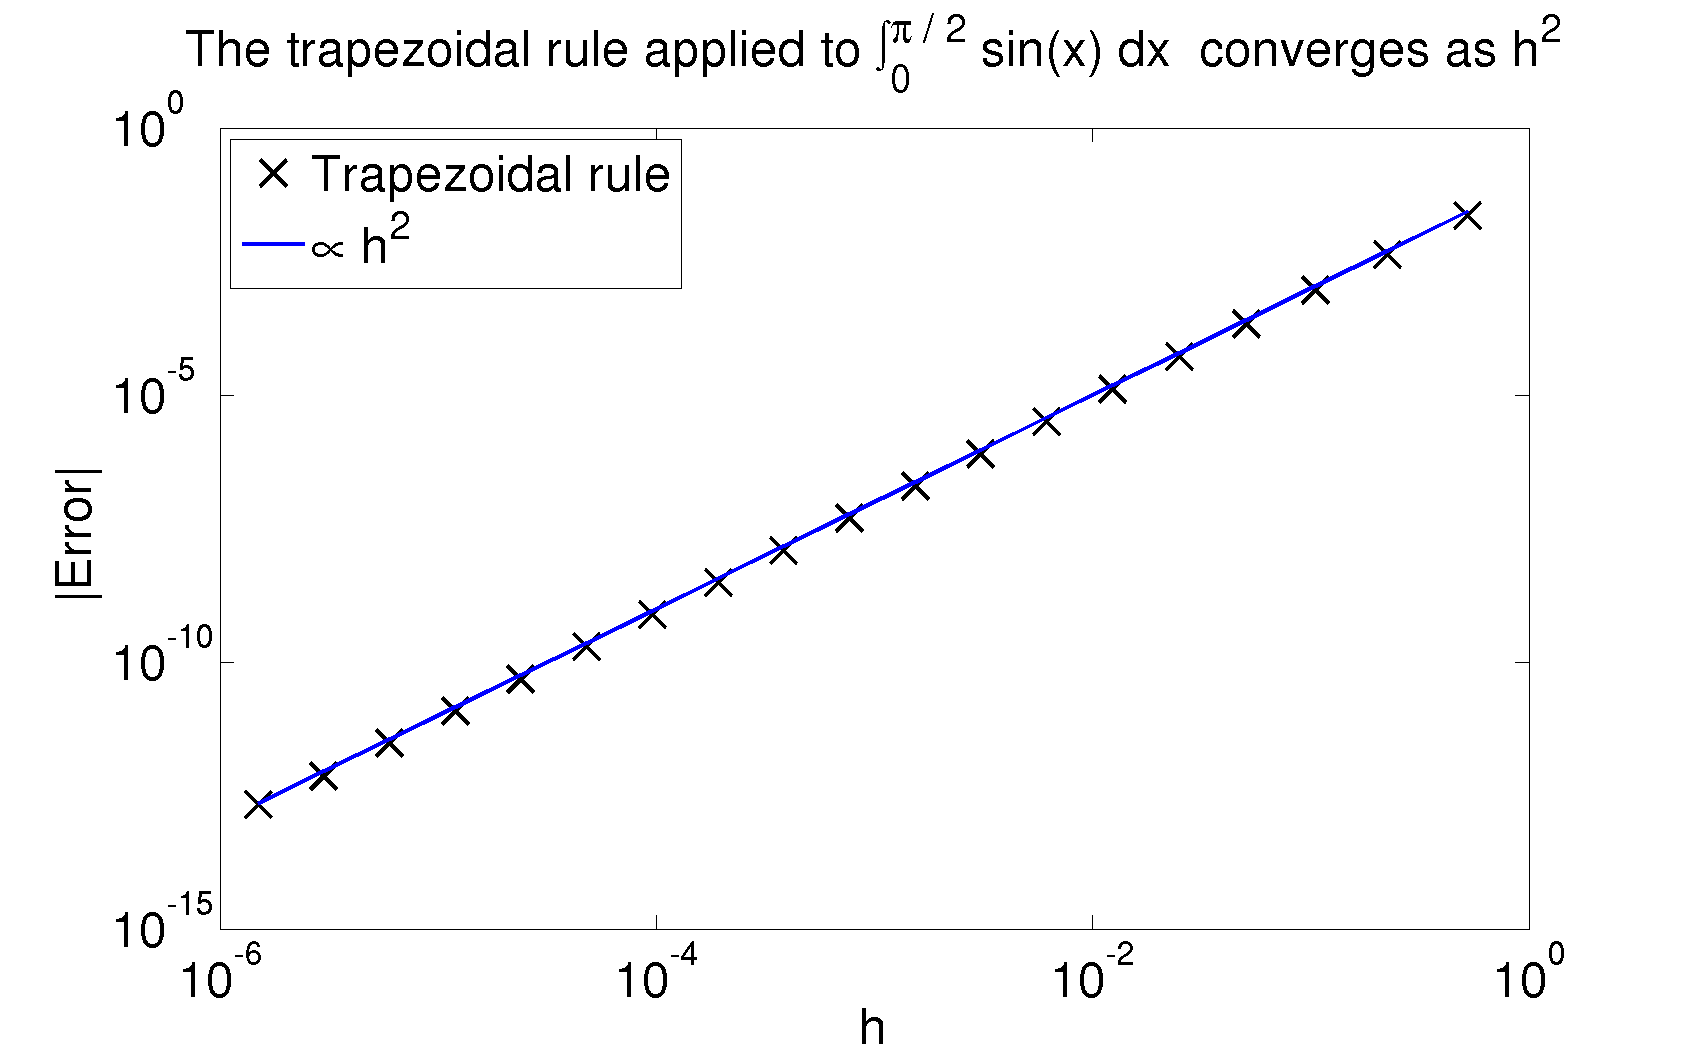
\includegraphics[width=0.8\textwidth]{figures/Trapezoidal1}
  \end{center}
  The example converges as expected with resolution.

\end{frame}

\section{Summary}

\subsection{Summary}

\begin{frame}
  \frametitle{Summary}

  \begin{itemize}
  \item When working with functions you have to decide how to
    represent the function using a finite amount of data.
  \item If you decide to do quadrature (integration) using that
    \begin{itemize}
    \item The value of the function is known at a finite number of nodes;
    \item The interpolating function is a polynomial
    \end{itemize}
    then you are using a Newton-Cotes formula.
  \item The trapezoidal rule interpolates the function using a linear
    polynomial (straight line).
  \item The composite trapezoidal rule breaks the interval into many
    small pieces and applies the trapezoidal rule to each.
  \item If each subinterval has the same width $h$ the trapezoidal
    rule is very simple and converges $\propto h^{2}$.
  \end{itemize}

\end{frame}

\end{document}



%%% Local Variables:
%%% mode: latex
%%% TeX-master: t
%%% End:
